\chapter{Parte Práctica}
\section{Ejercicio 1}
En este ejercicio se debe entrenar un modelo \textit{HoeffdingTree} con un flujo de datos generado con \textit{WaveformGenerator}, semilla inicializada a 2 y un millón de instancias. Tras esto se debe utilizar otro flujo generado con \textit{WaveformGenerator} utilizando como semilla el 4 y un millón de datos. Tras esto se debe probar el modelo \textit{HoeffdingAdaptiveTree} con los mismo paramétros. Dado que con un solo ejemplo no vale para saber que algoritmo es mejor que otro, se realizarán 10 pruebas con cada uno de los clasificadores y se estudiaran los resultados obtenidos.

Las sentencias necesarias para realizar lo anterior son las siguientes:
\vspace{0.06in}

\textit{java -cp moa.jar moa.DoTask ``EvaluateModel -m
(LearnModel -l trees.HoeffdingTree -s
(generators.WaveformGenerator -i 2) -m 1000000)
-s (generators.WaveformGenerator -i 4)``}

\textit{java -cp moa.jar moa.DoTask ``EvaluateModel -m
(LearnModel -l trees.HoeffdingAdaptiveTree -s
(generators.WaveformGenerator -i 2) -m 1000000)
-s (generators.WaveformGenerator -i 4)``}
\vspace{0.06in}


Las opciones que se pueden ver en las sentencias son las siguientes:
\begin{itemize}
	\item \textit{EvaluateModel} -m: para expecificar el modelo.
	\item \textit{LearnModel} -l: para expecificar modelo que se va a entrenar.
	\item \textit{LearnModel} -s: para el flujo de datos con el que se entrena el modelo.
	\item \textit{LearnModel} -m: para expecificar el número de instancias con el que se entrena el modelo.
	\item \textit{WaveformGenerator} -i: para expecificar la semilla con la que se inicializa el generador.
	\item \textit{EvaluateModel} -s: para expecificar el flujo de datos con el que se evalúa el modelo que ha sido entrenado.
\end{itemize}

Para realizar las pruebas con diferentes semillas se han creados dos scripts para automatizar el proceso. Tras esto se han mirado los resultados y se ha realizado un test para ver si existen diferencias entre ambos algoritmos.

\begin{figure}[H]
	\centering
	\subfigure[script para HoeffdingTree]{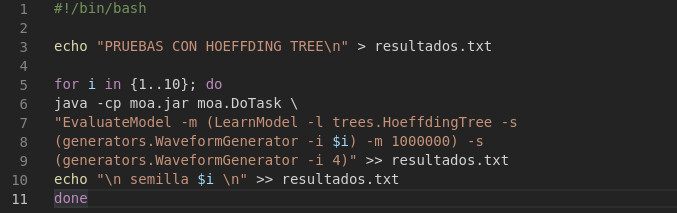
\includegraphics[width=80mm]{imagenes/script_hoeff}}
	\subfigure[script para HoeffdingAdaptiveTree]{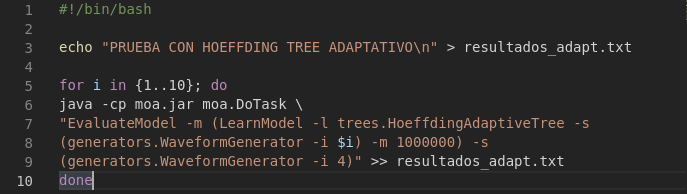
\includegraphics[width=80mm]{imagenes/script_hoeff_adapt}}
	\caption{Scripts para generar las pruebas de forma automática}
	\label{fig:scripts1}
\end{figure}

Los resultados obtenidos por los clasificadores son los siguientes.
\begin{table}[H]
	\begin{tabular}{lllll}
		\textbf{Semilla} & \textbf{Accuracy} & \textbf{Kappa} & \textbf{Accuracy Adaptive} & \textbf{Kappa Adaptive} \\ \hline
		1                & 84,509            & 76,765         & 84,521                     & 76,783                  \\
		2                & 84,512            & 76,77          & 84,474                     & 76,712                  \\
		3                & 84,59             & 76,887         & 84,416                     & 76,625                  \\
		4                & 84,666            & 77,001         & 84,465                     & 76,699                  \\
		5                & 84,481            & 76,723         & 84,262                     & 76,395                  \\
		6                & 84,342            & 76,514         & 84,368                     & 76,554                  \\
		7                & 84,799            & 77,2           & 84,271                     & 76,408                  \\
		8                & 84,153            & 76,231         & 84,243                     & 76,36                   \\
		9                & 84,641            & 76,963         & 84,478                     & 76,719                  \\
		10               & 84,578            & 76,869         & 84,326                     & 76,491                 
	\end{tabular}
\label{table:1}
\caption{Resultados pruebas ejercicio 1}
\end{table}

Como se puede ver los valores son muy similares, aún así se utilizará un test para confirmar que no hay diferencias de rendimiento entre ambos clasificadores.

\begin{figure}[H]
	\centering
	\subfigure[test de normalidad]{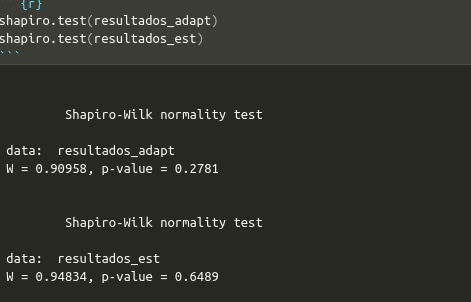
\includegraphics[width=40mm]{imagenes/normality_ej1}}
	\subfigure[test de wilcoxon]{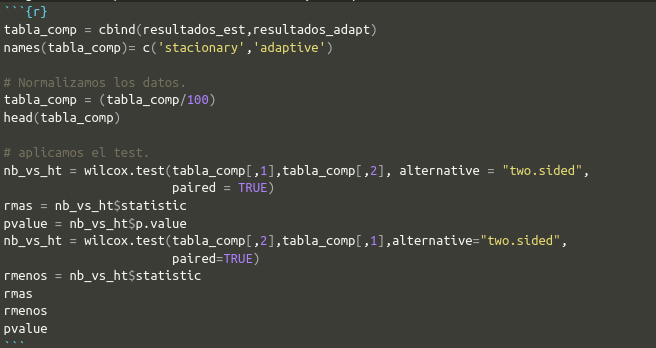
\includegraphics[width=65mm]{imagenes/wilc_ej1}	}
\end{figure}

El resultado del test de Wilcoxon es: 0.03710938

Por lo que se puede ver en los resultados, los dos algoritmos están ofreciendo los mismos resultados; esto puede ser posiblemente porque estamos entrenando ambos algoritmos de forma offline, por lo cual tanto HoeffdingTree como HoeffdingAdaptiveTree están aprendiendo sobre el mismo conjunto de datos y no son capaces de responder a cambios de concepto como el que tiene el flujo de datos generado con la semilla 4. Además, si realizamos un estudio sobre los resultados, el test muestra que existen diferencias significativas entre ambos algoritmos, pero después la diferencia entre la mediana de un algoritmo y otro son casi inexistentes.

\section{Ejercicio 2}
Para este ejercicio se debe hacer lo mismo que en el anterior pero cambiando el método de evaluación por \textit{InterleavedTestThenTrain}. A diferencia que en el ejercicio anterior, no se necesita entrenar un modelo, ya que el método de evaluación \textit{InterleavedTestThenTrain} primero testea los datos y después los utiliza para entrenar, por lo tanto está entrenando y testeando datos durante todo el proceso.Las sentencias necesarias para evaluar los modelos son los siguientes:
\vspace{0.06in}

\textit{java -cp moa.jar moa.DoTask \\
``EvaluateInterleavedTestThenTrain -l
trees.HoeffdingTree -s
(generators.WaveformGenerator -i 2)
-i 1000000 -f 10000`` > resultados\_online.txt}

\textit{java -cp moa.jar moa.DoTask \\
``EvaluateInterleavedTestThenTrain -l
trees.HoeffdingAdaptiveTree -s
(generators.WaveformGenerator -i 2)
-i 1000000 -f 10000`` > resultados\_online\_adative.txt}

Las opciones que se muestran para estas sentencias son las mismas que para el ejercicio anterior menos la opción -l de \textit{EvaluateInterleavedTestThenTrain}; esta función se utiliza  para evaluar un modelo con Test-Then-Train especificado mediante la opción -l. Las otras opciones que se pueden ver son -i que especifica el número de instancias totales con las que se evaluará el modelo y -f que especifica el número de instancias que llegan en cada momento.

Para realizar un estudio sobre ambos modelos; \textit{HoeffdingTree} y \textit{HoeffdingAdaptiveTree}, se han creado dos scripts para realizar pruebas con diferentes valores para la semilla de inicialización del generador \textit{WavefromGenerator}. Los scripts son los siguientes:

\begin{figure}[H]
	\centering
	\subfigure[script para HoeffdingTree]{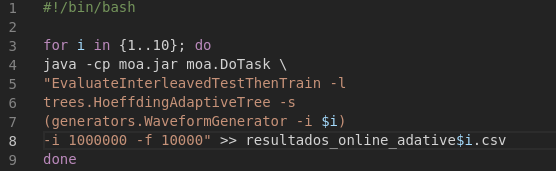
\includegraphics[width=80mm]{imagenes/script_online_hoeff}}
	\subfigure[script para HoeffdingAdaptiveTree]{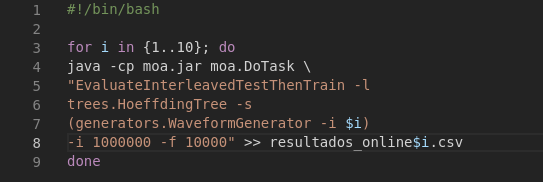
\includegraphics[width=80mm]{imagenes/script_online_adapt}}
	\caption{Scripts para generar las pruebas de forma automática con EvaluateInterleavedTestThenTrain}
	\label{fig:scripts2}
\end{figure}

Los resultados obtenidos por los clasificadores son los siguientes.
\begin{table}[H]
	\begin{tabular}{lllll}
		\textbf{Semilla} & \textbf{Accuracy} & \textbf{Accuracy Adaptive} & \textbf{Kappa} & \textbf{Kappa Adaptive} \\ \hline
		1                & 83,8903           & 83,8042                    & 75,83623569    & 75,7071683              \\
		2                & 83,7851           & 83,7313                    & 75,67749802    & 75,5967623              \\
		3                & 83,8876           & 83,7875                    & 75,82954147    & 75,6792025              \\
		4                & 84,0451           & 83,7961                    & 76,06946036    & 75,69604195             \\
		5                & 83,8402           & 83,7144                    & 75,75999473    & 75,57128698             \\
		6                & 83,9062           & 83,8406                    & 75,85905507    & 75,76071273             \\
		7                & 83,8867           & 83,7784                    & 75,82927699    & 75,66688337             \\
		8                & 83,8687           & 83,8968                    & 75,8028419     & 75,84506754             \\
		9                & 83,7875           & 83,8282                    & 75,6817212     & 75,7427829              \\
		10               & 83,8479           & 83,9                       & 75,77149369    & 75,84955066            
	\end{tabular}
\label{table:2}
\caption{Resultados pruebas ejercicio 2}
\end{table}

Al igual que en el ejercicio anterior, no parece haber diferencias entre los dos algoritmos; aún así se realizará un test para ver si existen diferencias entre ellos.


Para ver si hay diferencias significativas entre ambos algoritmos, cargaremos los datos y comprobaremos si existen diferencias significativas.La forma de comprobar la normalidad de las soluciones y el test se realiza de la misma forma que en el ejercicio anterior. Al igual que en el ejercicio anterior, los resultados nos siguen una distribución normal, por lo que se utilizará el test de Wilcoxon para comprobar si hay diferencias de rendimiento entre ambos algoritmos.

Por los resultados del test (0.02734375), debería de haber diferencias significativas, pero al hacer la media de la precisión de ambos algoritmos se puede ver que son casi iguales, por lo que descartaremos la hipótesis del test y diremos que no hay diferencias entre los algoritmos. Es normal que no haya diferencias significativas entre los modelos, ya que a no ser que en el flujo de datos haya un cambio de concepto ambos modelos se comportan de forma igual.

\section{Ejercicio 3}
Para este ejercicio se debe entrenar un \textit{HoeffdingTree} online con test-then-train sobre 2M de instancias y freq. muestreo de 100k generando los datos con un generador \textit{RandomRBFGeneratorDrift}, con semilla aleatoria igual a 1 para generación de instancias, generando 2 clases, 7 atributos, 3 centroides, drift en todos los centroides y velocidad de cambio igual a 0.001. También se probará el modelo \textit{HoeffdingAdaptiveTree}. Las sentencias necesarias para ejecutar ambos modelos son las siguientes:
\vspace{0.06in}

\textit{java -cp moa.jar moa.DoTask \\``EvaluateInterleavedTestThenTrain -l trees.HoeffdingTree -s\\
(generators.RandomRBFGeneratorDrift -s 0.001 -k 3 -r 1 -i 1 -a 7 -n 3)
-i 2000000 -f 100000``
}

\textit{java -cp moa.jar moa.DoTask \\``EvaluateInterleavedTestThenTrain -l trees.HoeffdingAdaptiveTree -s\\
(generators.RandomRBFGeneratorDrift -s 0.001 -k 3 -r 1 -i 1 -a 7 -n 3)
-i 2000000 -f 100000``}

\vspace{0.06in}

Las nuevas opciones que hay a diferencia de los ejercicios anteriores son las opciones del generador \textit{RandomRBFGeneratorDrift}. La opción -s especifica la velocidad de cambio en los centroides, la opción -r especifica la semilla para la generación de modelos, la opción -i especifica la semilla para la generación de instancias, la opción -a especifica el número de atributos que tiene cada instancia, la opción -k especifica el número de centroides que cambian y la opción -n especifica el número de centroides del flujo de datos.
\newline

Para realizar un estudio sobre el comportamiento de los algoritmos, se ha utilizado la GUI de MOA para poder ver una gráfica sobre la precisión de los modelos sobre el flujo de datos que se genera. Para este ejercicio se han utilizado 3 semillas diferentes para cada uno de los modelos, los resultados obtenidos son los siguientes.

\begin{figure}[H]
	\centering
	\subfigure[HoeffdingTree]{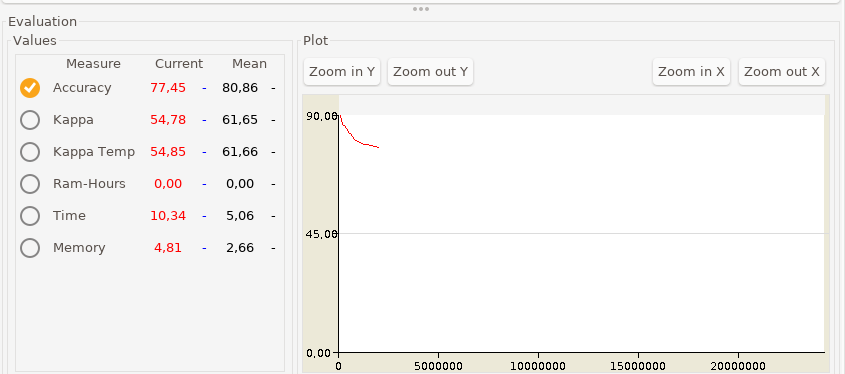
\includegraphics[width=70mm]{imagenes/rbf_drift_s1}}
	\subfigure[HoeffdingAdaptiveTree]{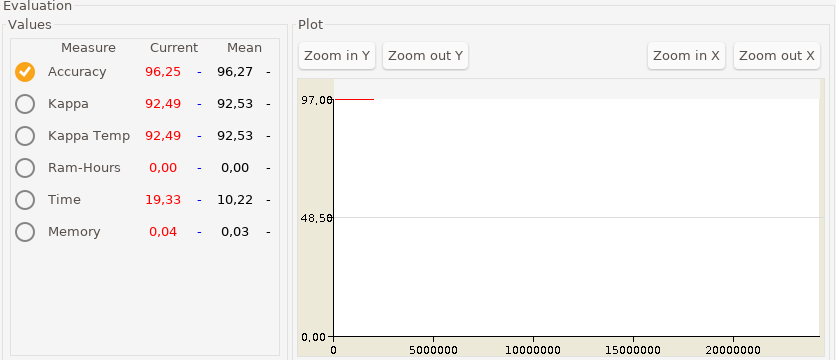
\includegraphics[width=70mm]{imagenes/rbf_drift_s1_adapt}}
	\caption{Resultados InterleavedTestThenTrain con semilla 1}
	\label{fig:res31}
\end{figure}

\begin{figure}[H]
	\centering
	\subfigure[HoeffdingTree]{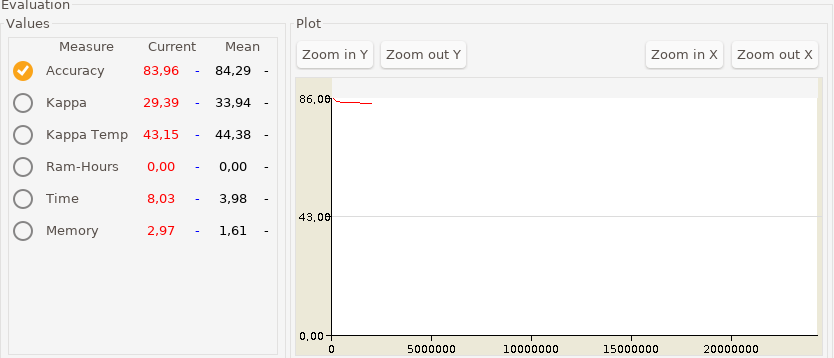
\includegraphics[width=70mm]{imagenes/rbf_drift_s2}}
	\subfigure[HoeffdingAdaptiveTree]{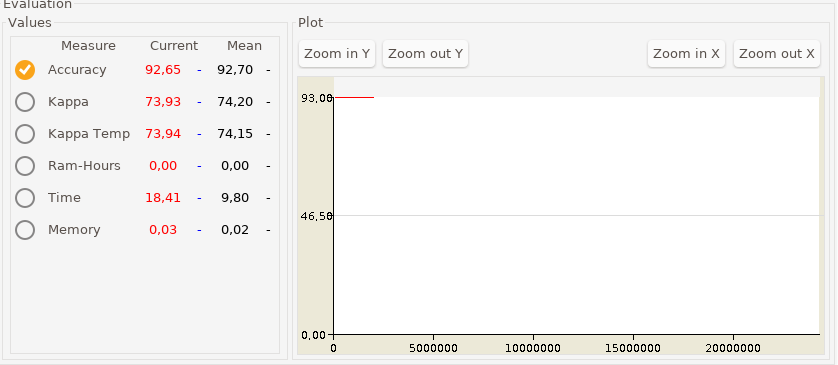
\includegraphics[width=70mm]{imagenes/rbf_drift_s2_adapt}}
	\caption{Resultados InterleavedTestThenTrain con semilla 2}
	\label{fig:res32}
\end{figure}

\begin{figure}[H]
	\centering
	\subfigure[HoeffdingTree]{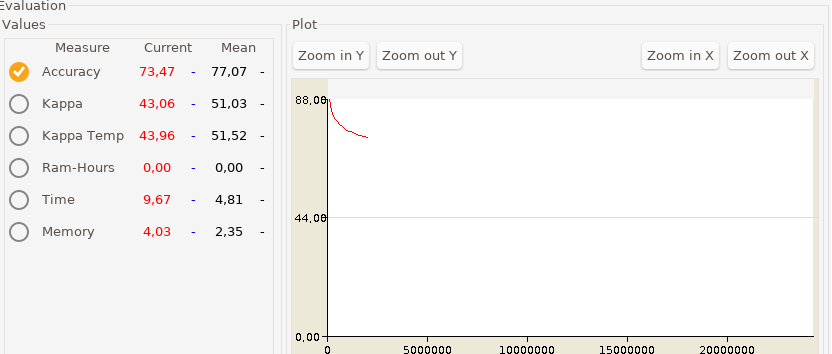
\includegraphics[width=70mm]{imagenes/rbf_drift_s3}}
	\subfigure[HoeffdingAdaptiveTree]{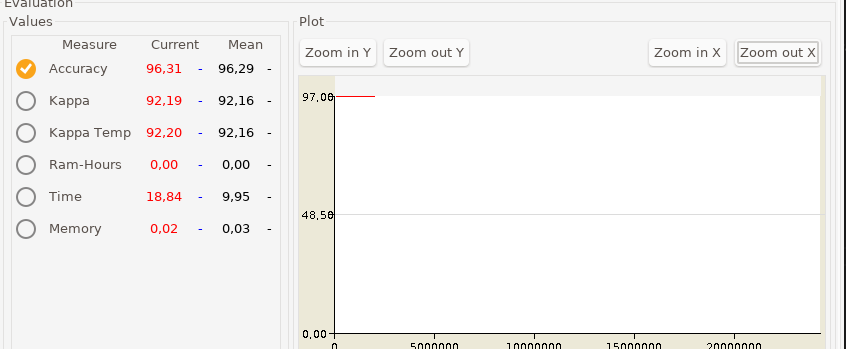
\includegraphics[width=70mm]{imagenes/rbf_drift_s3_adapt}}
	\caption{Resultados InterleavedTestThenTrain con semilla 3}
	\label{fig:res33}
\end{figure}
Si nos fijamos en los resultados que se pueden ver en las imágenes
de la GUI de MOA, se puede ver que el clasificador \textit{HoeffdingTree} obtiene
peores resultados que su versión adaptativa, esto es así porque el
algoritmo \textit{HoeffdingTree} no está preparado para los cambios de concepto,
por ello cuando hay un cambio de concepto la precisión del algoritmo
baja bastante. En cambio, el clasificador \textit{HoeffdingAdaptiveTree} sí que
está preparado para detectar cambios de concepto, para ello utiliza el
método \textit{ADWIN}, una vez detectado el cambio de concepto puede re-entrenar
el árbol, podar ciertas ramas que ya no sirvan, etc. Por ello, no
sufre una bajada en la precisión como le pasa al algoritmo \textit{HoeffdingTree}
y es apto para clasificación con flujos que tienen cambios de concepto.

\section{Ejercicio 4}
Igual que el modelo anterior, pero utilizando la función Prequential en vez de la función TestThenTrain. El método de evaluación Prequential testea con cada ejemplo que se le va entrando y después reentrena el modelo; utiliza una ventana para ir olvidando ejemplos antiguos y centrarse en ejemplos nuevos. La sentencias necesarias para evaluar es la siguiente.
\vspace{0.06in}

\textit{java -cp moa.jar moa.DoTask \\ ``EvaluatePrequential -l trees.HoeffdingTree
-e (WindowClassificationPerformanceEvaluator -w 1000) -s
(generators.RandomRBFGeneratorDrift -s 0.001 -k 3 -r 1 -i 1 -a 7 -n 3)
-i 2000000``}

\textit{java -cp moa.jar moa.DoTask \\ ``EvaluatePrequential -l trees.HoeffdingAdaptiveTree
-e (WindowClassificationPerformanceEvaluator -w 1000) -s
(generators.RandomRBFGeneratorDrift -s 0.001 -k 3 -r 1 -i 1 -a 7 -n 3)
-i 2000000``}

Al igual que en el ejercicio anterior, se han hecho pruebas con 3 semillas diferentes. Los resultados son los siguientes.

\begin{figure}[H]
	\centering
	\subfigure[HoeffdingTree]{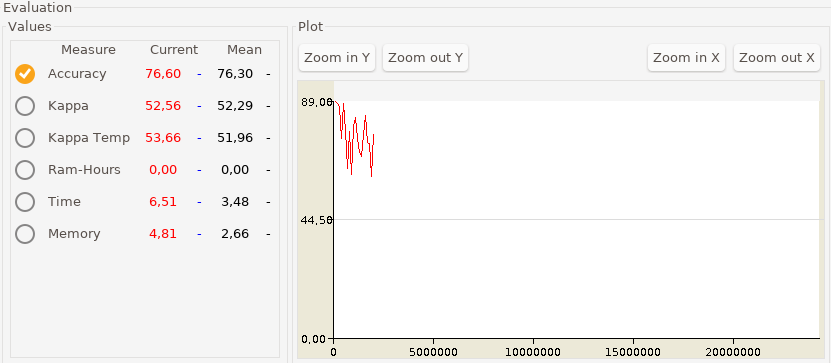
\includegraphics[width=70mm]{imagenes/prequential_s1}}
	\subfigure[HoeffdingAdaptiveTree]{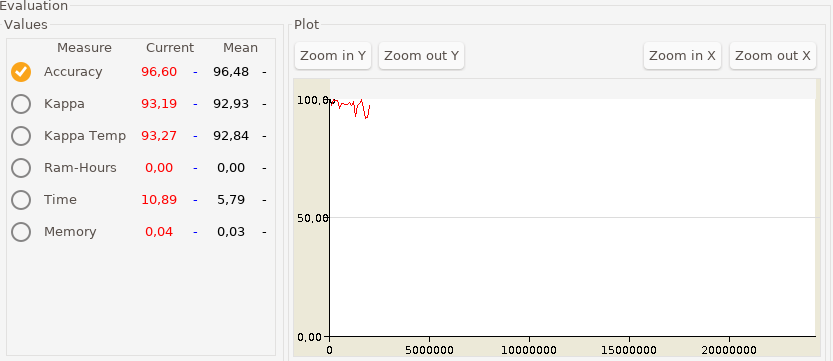
\includegraphics[width=70mm]{imagenes/prequential_adaptive_s1}}
	\caption{Resultados Prequential con semilla 1}
	\label{fig:res41}
\end{figure}

\begin{figure}[H]
	\centering
	\subfigure[HoeffdingTree]{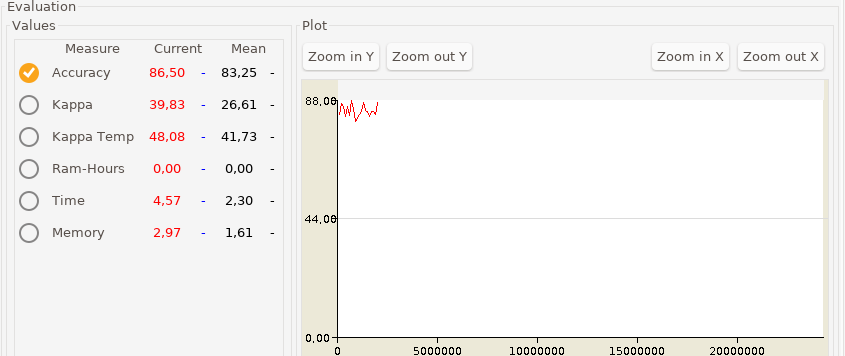
\includegraphics[width=70mm]{imagenes/prequential_s2}}
	\subfigure[HoeffdingAdaptiveTree]{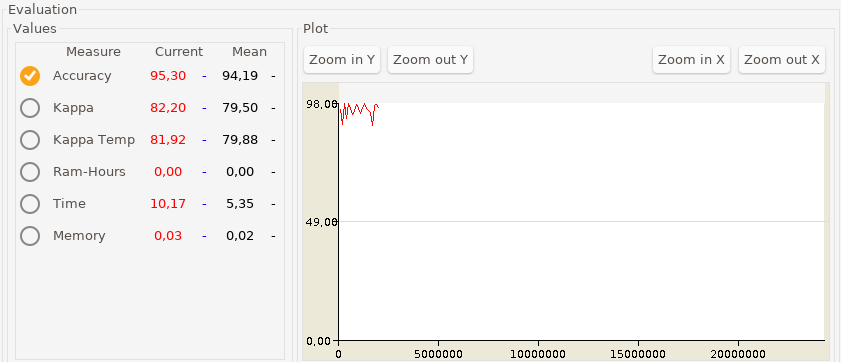
\includegraphics[width=70mm]{imagenes/prequential_adaptive_s2}}
	\caption{Resultados Prequential con semilla 2}
	\label{fig:res42}
\end{figure}

\begin{figure}[H]
	\centering
	\subfigure[HoeffdingTree]{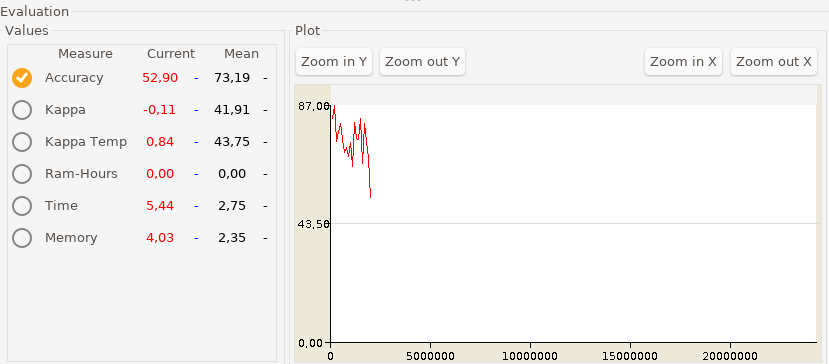
\includegraphics[width=70mm]{imagenes/prequential_s3}}
	\subfigure[HoeffdingAdaptiveTree]{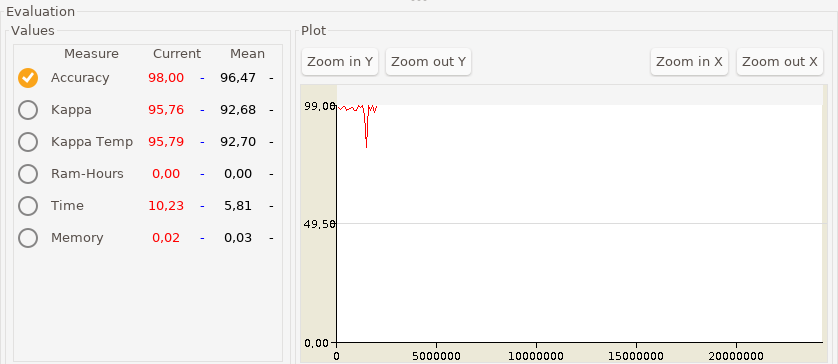
\includegraphics[width=70mm]{imagenes/prequential_adaptive_s3}}
	\caption{Resultados Prequential con semilla 3}
	\label{fig:res43}
\end{figure}
\vspace{0.06in}

Realizando pruebas con ambos algoritmos, se puede ver una gran diferencia
entre cada uno de los algoritmos. El clasificador \textit{HoeffdingTree} sufre una
gran bajada en la precisión cuando llega un cambio de concepto, y para
cuando puede recuperarse vuelve a haber otro cambio de concepto; por lo
que su rendimiento vuelve a bajar. Por otro lado, el clasificador
\textit{HoeffdingAdaptiveTree} al detectar los cambios de concepto, tiene pequeñas
bajadas en la precisión de las cuales se recupera rápidamente. Por lo tanto
para este tipo de flujo de datos el clasificador \textit{HoeffdingAdaptiveTree}
es mejor que \textit{HoeffdingTree}.

\section{Ejercicio 5}
Repetir el ejercicio anterior cambiando el modelo con \textit{SingleClassfierDrift},
utilizando el modelo \textit{HoeffdingTree}. Este método, reemplaza el clasificador
cuando se detecta un cambio de concepto. La sentencia necesaria para ejecutar
la evaluación del modelo es la siguiente:

\textit{java -cp moa.jar moa.DoTask \\ ``EvaluateInterleavedTestThenTrain -l
(drift.SingleClassifierDrift -l trees.HoeffdingTree) -s
(generators.RandomRBFGeneratorDrift -s 0.001 -k 3 -r 1 -i 1 -a 7 -n 3)
-i 2000000 -f 100000``}

Para la modificación con el modelo HoeffdingAdaptiveTree habría que utilizar
la siguiente sentencia:
\textit{java -cp moa.jar moa.DoTask \\ ``EvaluateInterleavedTestThenTrain -l
(drift.SingleClassifierDrift -l trees.HoeffdingAdaptiveTree) -s
(generators.RandomRBFGeneratorDrift -s 0.001 -k 3 -r 3 -i 3 -a 7 -n 3)
-i 2000000 -f 100000``}

La única opción nueva con respecto al resto de ejercicios es la opción -l de la acción \textit{SingleClassifierDrift} que especifica que modelo tiene que utilizar este método.

Al igual que en el ejercicio 3, se han ejecutado los algoritmos con tres semillas diferentes para el generador \textit{RandomRBFGeneratorDrift}. Los resultados obtenidos por los clasificadores son los siguientes.

\begin{figure}[H]
	\centering
	\subfigure[HoeffdingTree]{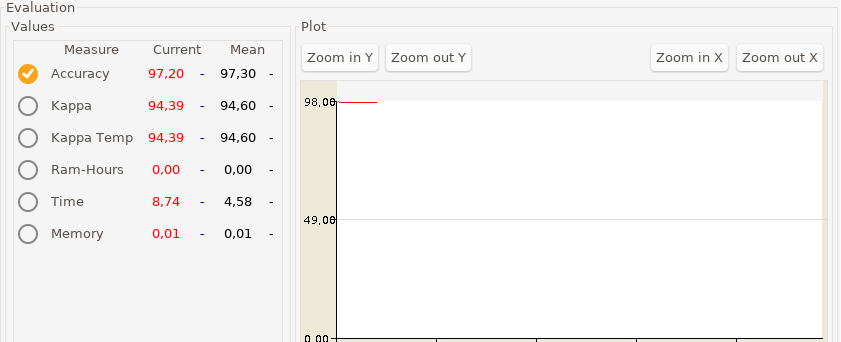
\includegraphics[width=70mm]{imagenes/singledrift_hoff}}
	\subfigure[HoeffdingAdaptiveTree]{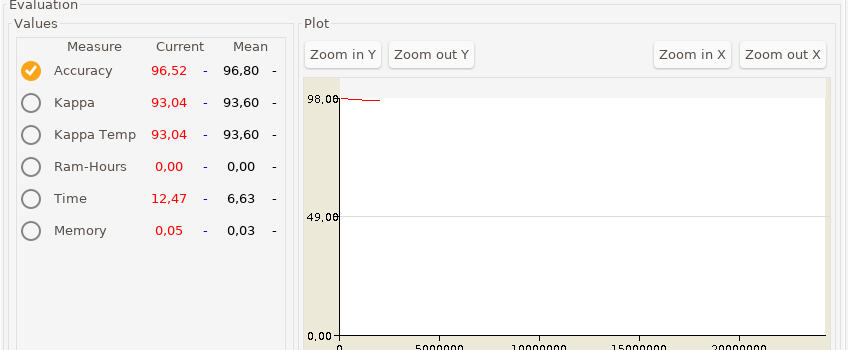
\includegraphics[width=70mm]{imagenes/singledrift_hoffadp}}
	\caption{Resultados SingleClassifierDrift con semilla 1}
	\label{fig:res51}
\end{figure}

\begin{figure}[H]
	\centering
	\subfigure[HoeffdingTree]{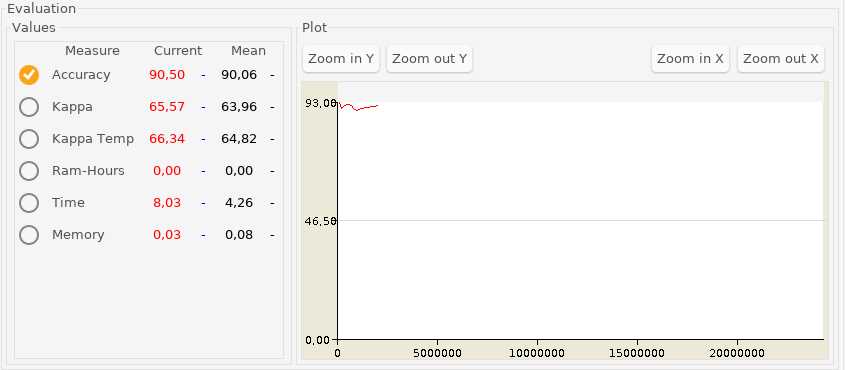
\includegraphics[width=70mm]{imagenes/singledrift_hoffs2}}
	\subfigure[HoeffdingAdaptiveTree]{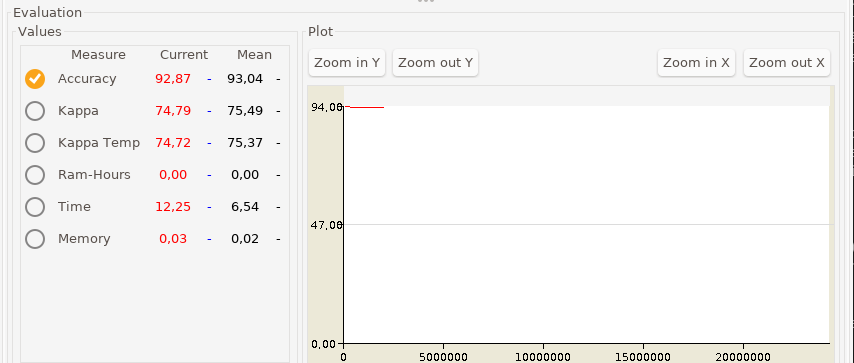
\includegraphics[width=70mm]{imagenes/singledrift_hoffadps2}}
	\caption{Resultados SingleClassifierDrift con semilla 2}
	\label{fig:res52}
\end{figure}

\begin{figure}[H]
	\centering
	\subfigure[HoeffdingTree]{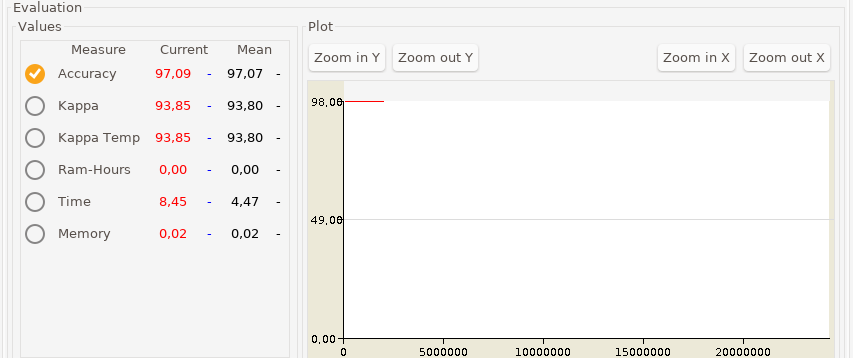
\includegraphics[width=70mm]{imagenes/singledrift_hoffs3}}
	\subfigure[HoeffdingAdaptiveTree]{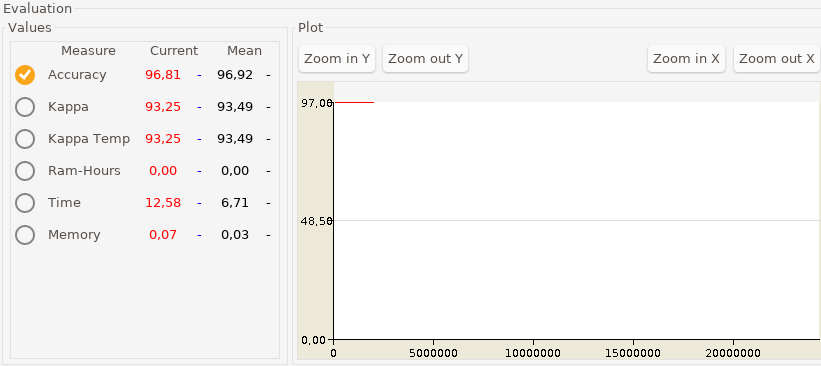
\includegraphics[width=70mm]{imagenes/singledrift_hoffadps3}}
	\caption{Resultados SingleClassifierDrift con semilla 3}
	\label{fig:res53}
\end{figure}

Como se puede ver en las gráficas obtenidas en la GUI de MOA, la precisión
de ambos clasificadores es la misma. A diferencia del ejercicio 2.3,
se utiliza un modelo \textit{SingleClassfierDrift}; por ello, el clasificador se
cambia cuando se detecta un cambio de concepto. Por lo tanto, cada vez que
hay un cambio de concepto se crea un nuevo modelo, tanto para \textit{HoeffdingTree}
como para \textit{HoeffdingAdaptiveTree} y entonces el modelo \textit{HoeffdingAdaptiveTree} se comporta como el modelo \textit{HoeffdingTree} ya que este no detecta el cambio
de concepto. En cambio, en el ejercicio 4 y en el ejercicio 3 sí que hay una diferencia de rendimiento entre ambos clasificadores, ya que el clasificador \textit{HoeffdingAdaptiveTree} puede detectar los cambios de concepto y el otro no. Como similitud en los tres ejercicios está el tipo de flujo que se ha utilizado para comparar el rendimiento de los clasificadores, que siempre ha sido el generado por el generador \textit{RandomRBFGeneratorDrift} con las mismas semillas y parámetros.

